\section{Experimental Results}
\label{sec:experiments}
% Experimental results

We trained MacroQ learning agents on several standard domains, and
measured the cumulative return obtained using the following option
generation schemes: 
\begin{itemize}
   \item \textbf{None}: No options were used.
   \item \textbf{Random}: Options were generated by randomly connecting
     two nodes in the domain (this is equivalent to $P_0$).
   \item \textbf{Betweenness}: As a representative of bottleneck-based
     schemes, options were generated to take any node to a local maxima
     of betweenness centrality, as described in \cite{Simsek2008}. 
   \item \textbf{Small World}: Options were generated randomly
     connecting two nodes of the domain using an inverse square law, as
     described in \secref{sec:theory}.
\end{itemize}

Each experiment, unless mentioned otherwise, was run for $10$ randomly
generated tasks in the domain; each task ran for $40,000$ epochs, and
was averaged over an ensemble of $20$ agents.

\subsection{Optimal Options}
The agents were run on the following three domains using the algorithm
sketched in \secref{sec:theory}:
\begin{itemize}
   \item \textbf{Arbitrary Navigation}: The agent must reach an
     arbitrary goal state in an obstacle-free $x \times y$ grid-world. 
   \item \textbf{Rooms}: The agent must navigate a floor plan with
     4 rooms to reach an arbitrary goal state.
   \item \textbf{Taxi}: This is the domain described in
     \exref{example:taxi}.
\end{itemize}

Optimal policies were given to the options generated according to the
schemes described above. 

\begin{table}
 \centering
 \begin{tabular}{ r | r r r }
             & Arbt. Navi           & Rooms               & Taxi                  \\ \hline
   None      & -31.82               &  -1.27              & -16.90                \\
   Random    & -31.23               & -10.76              & -18.83                \\
   Betw.     & -18.28               & -8.94               &  {\bf 80.48}          \\
   Sm-W      & {\bf -14.24 [$r=4$]} & {\bf 8.54[$r=2$]}   &   0.66 [$r=0.75$]     \\
 \end{tabular}
 \caption{Cumulative Return}
 \label{tbl:optimal-returns}
\end{table}

The results of these experiments are summarised in
Table \autoref{tbl:optimal-returns}. Small world options perform significantly
better than the other schemes in navigation-oriented tasks like Rooms or
Arbitrary Navigation. In the Taxi domain, options generated by the
betweenness scheme outperform the small world options. This is expected
because the goal states in this domain lie at betweenness maxima.

\begin{figure}[th]
  \centering
    \includegraphics[width=2.4in]{figures/rooms-options}
    \label{fig:rooms-options}
    \caption{Rooms: Options learnt}
\end{figure}

\begin{figure}[th]
  \centering
    \includegraphics[width=3in]{figures/rooms-return-200}
    \label{fig:rooms-return}
    \caption{Rooms: Cumulative Return with 200 options}
\end{figure}

Some of the small world options preferred in Rooms domain are shown in
\figref{fig:rooms-options}. The graph shows several examples of options
that compose together to arrive near the goal state. We have also
plotted the learning behaviour in \figref{fig:rooms-return}. 

\begin{figure}[th]
  \centering
      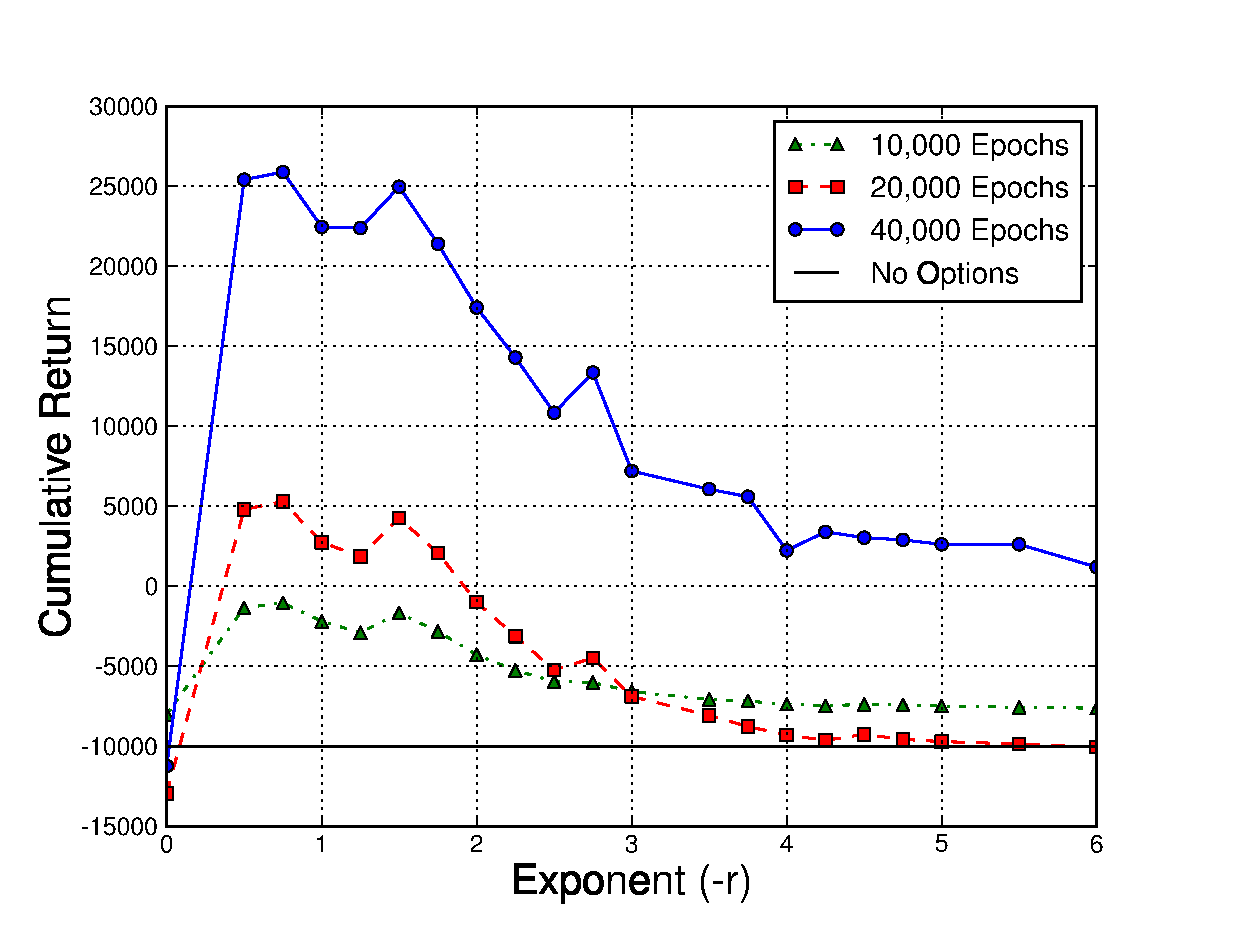
\includegraphics[width=3in]{figures/rooms-exp}
      \label{fig:rooms-exp}
    \caption{Rooms: $r$ vs Cumulative Return}
\end{figure}

\subsection{Sensitivity of $r$}
We do not yet have a clear understanding of how the exponent $r$ should
be chosen. \figref{fig:rooms-exp} plots $r$ versus the cumulative return
on the Rooms domain. The performance of the agent without options after
$20,000$ epochs is also plotted for reference. There is a range of $r$
($\approx 0.75$ to $1.5$) with good performance, after which the
performance steadily drops. This behaviour is easily explained; as the
exponent goes up, the small world options generated are very short, and
do not help the agent get nearer to the maximal value state. The optimal
range of $r$ is slightly counter-intuitive because the Rooms domain is
a two dimensional lattice with some edges removed. As a consequence of
the reduced connectivity, and perhaps due to stochastic factors, longer
range options are preferred.

\begin{figure}[th]
  \centering
    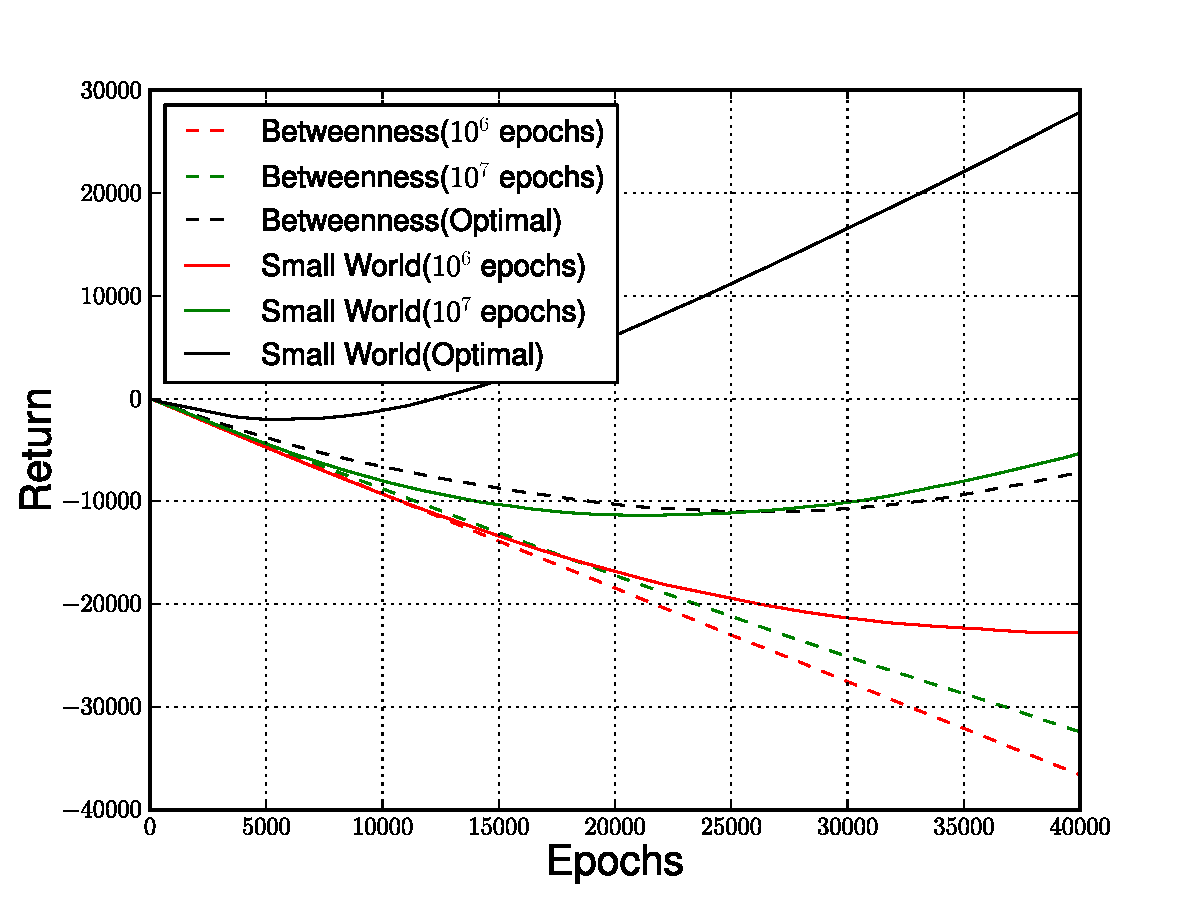
\includegraphics[width=3in]{figures/rooms-learnt-200}
      \label{fig:rooms-learnt}
    \caption{Rooms: Options Learnt on a Budget}
\end{figure}

\subsection{Options Learnt on a Budget}
In \secref{sec:algo}, we describe an algorithm to construct small world
options efficiently when given a limited number of learning epochs. We
compared the performance of these options with betweenness options
learnt similarly, and have plotted our results in
\figref{fig:rooms-learnt}. Despite using many more
options, the small world options thus created significantly outperform
betweenness options learnt with the same budget, and are even comparable
to the optimal betweenness options.

